\documentclass{school-22.101-notes}
\date{November 7, 2011}

\begin{document}
\maketitle



%%%%%%%%%%%%%%%% Spin-orbit Coupling %%%%%%%%%%%%%
\topic{Spin Orbital Coupling} \label{spin-orbit-coupling}
\subtopic{Potential with Spin-Orbit Coupling}
Our previous attempts suggest that single particle interaction is missing something fundamental. Thus we add the interaction between the orbital angular momentum and the intrinsic spin angular momentum of nucleon: 
\eqn{ V_{\mathrm{nuc}} (r) = V_0 (r) + V_{\mathrm{so}} (r) \frac{\lhat \cdot \shat}{\hbar^2} }
Notice:
\begin{itemize}
\item $\lhat, \shat$ are operators on a single nucleon; 
\item the $\frac{\lhat \cdot \shat}{\hbar^2}$ term could give the proper separation of the sub-shells;
\item Adding spin-orbit coupling does not destroy the physical content of the potential as the intermediate potential is a good guess for how the nuclear potential should look like; 
\item \textcolor{blue}{the interaction is NOT spherically symmetric.}
\end{itemize} 

\begin{align}
\expect{\lhat \cdot \shat} &= \frac{\hbar^2}{2} \left[ j(j+1) - l(l+1) - \frac{3}{4} \right] =
\begin{dcases*}
- \frac{\hbar^2}{2} (l+1) & for $j = l-\frac{1}{2}$. \\ 
\frac{\hbar^2}{2} l & for $j = l + \frac{2}{2}$. 
\end{dcases*} 
\\
V_{\mathrm{nuc}} (r) &= 
\begin{dcases*}
V_0 - \frac{l+1}{2} V_{\mathrm{so}} & for $j = l-\frac{1}{2}$. \\ 
V_0 + \frac{l}{2} V_{\mathrm{so}} & for $j = l + \frac{2}{2}$. \\
\end{dcases*}
\end{align}
Keep in mind that $V_0 < 0, V_{\mathrm{so}} < 0$, so 
\begin{itemize}
\item $j = l+\frac{1}{2}$: pushes the well and the energy levels down (lower), more tightly bound; the attractive well is more attractive; 
\item $j = l - \frac{1}{2}$: pushes the well and the energy levels higher (up), more weakly bound.  
\end{itemize}

\subtopic{Consequences of Spin-orbit Coupling}
\begin{enumerate}
\item Each of the original $l$ level would be spitted into two states $j= l \pm \frac{1}{2}$ as in Figure~\ref{s-o-coupling}. Notice the total number of states preserved even though degeneracy is not based on $m_l, m_s$ in this new notation. We use spectroscopic notation $nl_j$.  
\begin{figure}[h!]
    \centering
    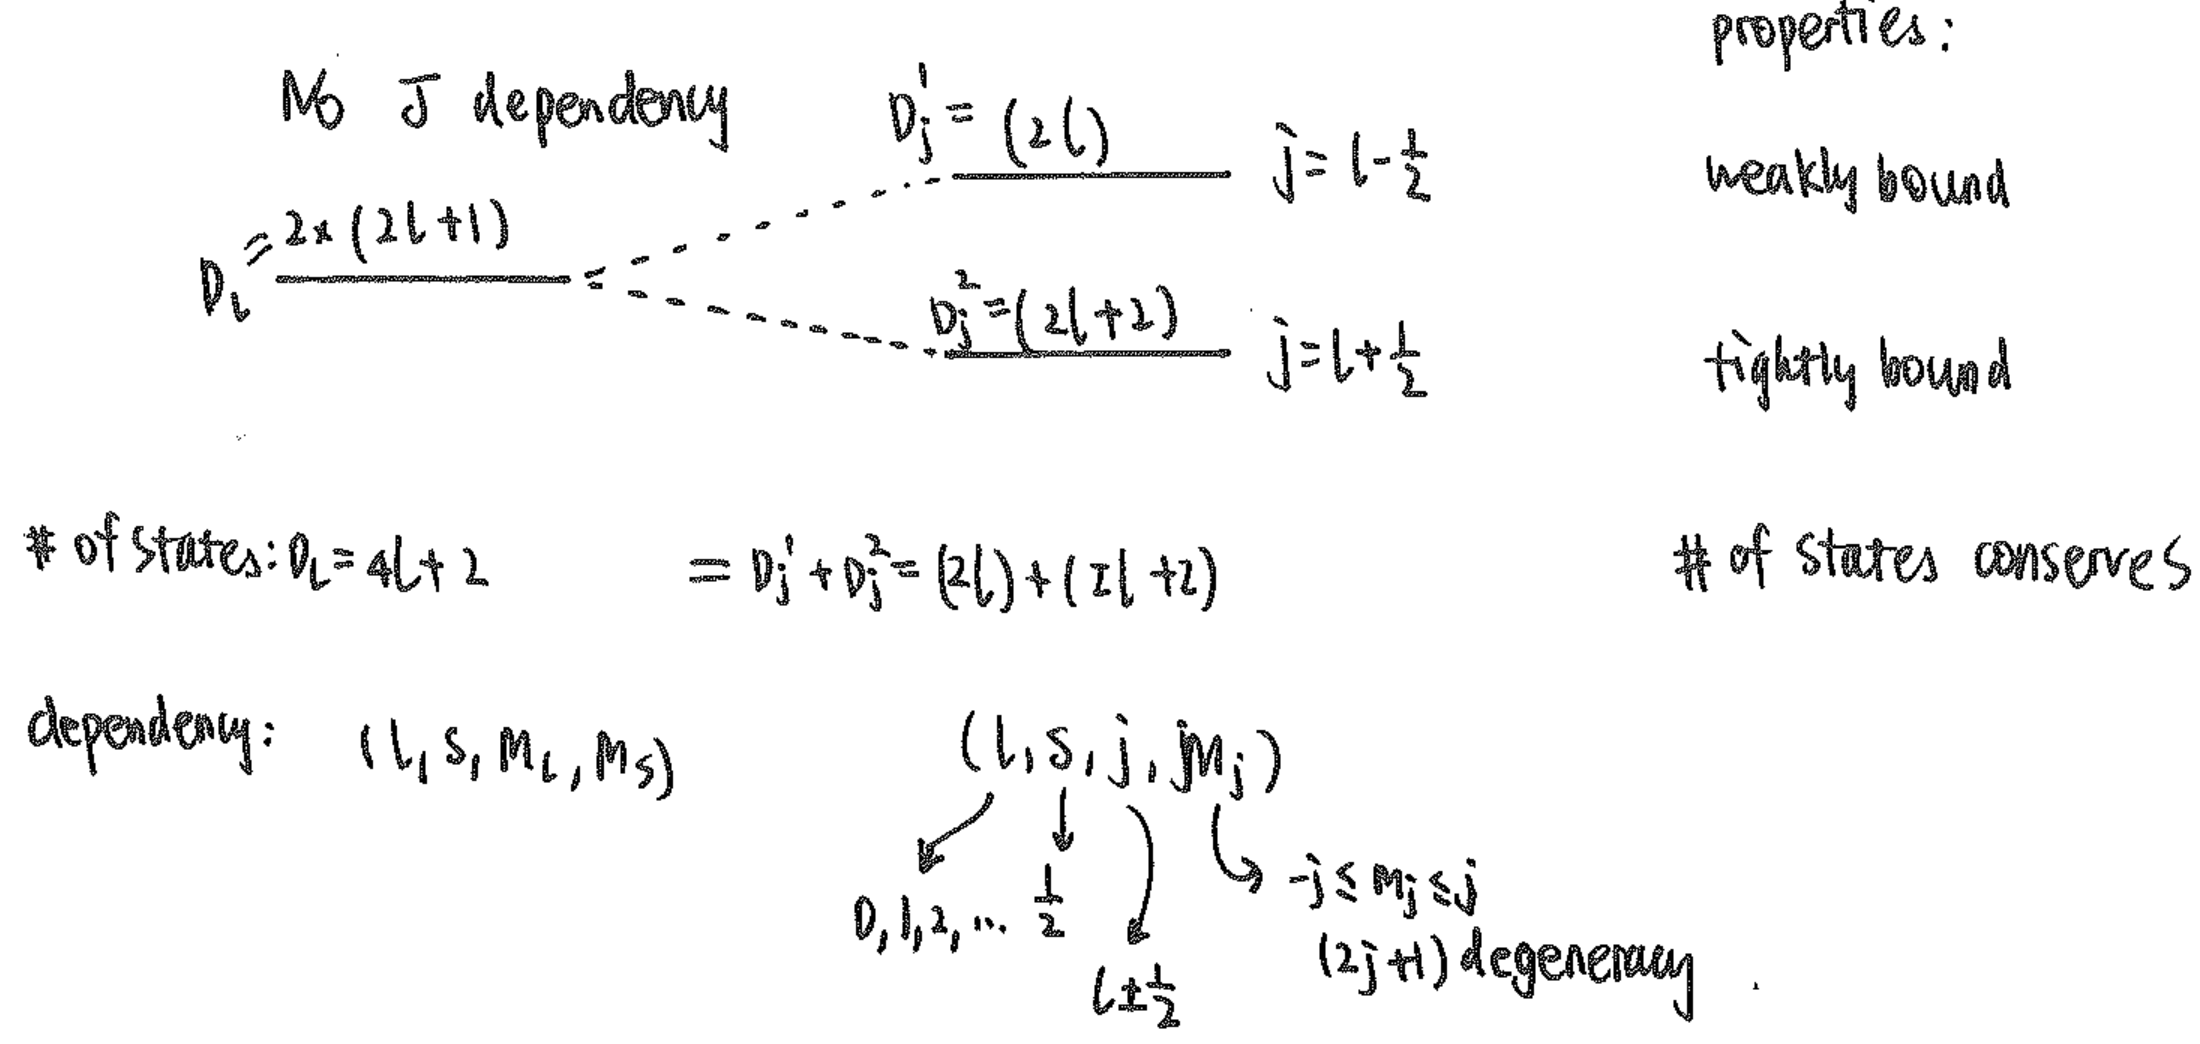
\includegraphics[width=4.6in]{images/shell/spin-orbit-coupling.png}
    \caption{Spin-Orbit Coupling, Splitting the Original $l$ Level into Two States}
    \label{s-o-coupling}
\end{figure}

\item The $j=l-\frac{1}{2}$ state makes the well shallower, making the state more weakly bound; the $j=l+\frac{1}{2}$ staet makes the well deeper, making the state more tightly bound. 
\begin{figure}[h!]
    \centering
    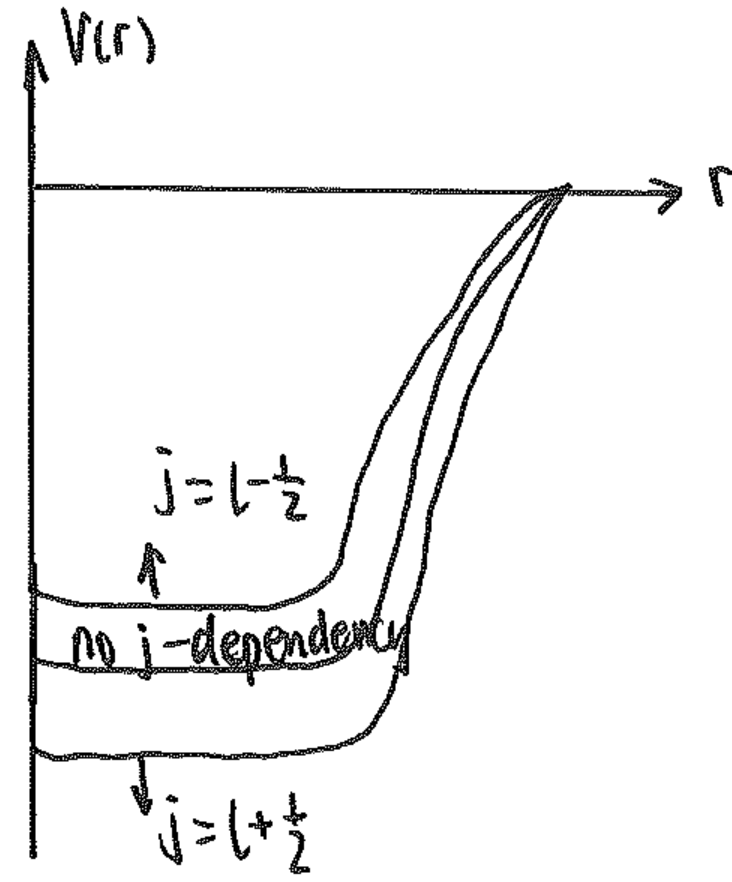
\includegraphics[width=1.5in]{images/shell/spin-orbit-coupling-potential.png}
    \caption{Potential Shifts after Applying Spin-Orbit Coupling}
\end{figure}

\item For a pair of states with $l>0$, the energy splitting difference increases with increasing $l$:
\eqn{ \Delta E = \expect{ \lhat \cdot \shat }_{j = l+\frac{1}{2} } - \expect{ \lhat \cdot \shat }_{j = l-\frac{1}{2} } = \frac{\hbar^2}{2} (2l+1) }
The physical interpretation of the this is that states with larger $l$ values split more; for instance, $1f$ state split more than than $2p$. In the deuteron example, $l=0$, hence we do not consider spin-orbit coupling. 
\end{enumerate}


\subtopic{Correction to the Intermediate Form Potential Shell Model}
\textcolor{blue}{Splitting of highest $l$ (recall larger $l$ results in larger $\Delta E$) at each oscillator level leads to re-joining of new j-levels with the top of the lower shell, and accounts for all the magic numbers.} Even the non-existing 184 is predicted. This founding leads to a Nobel Prize. 
\begin{enumerate}
\item $n=3$ oscillator level, the induced $1f_{7/2}$ reduces 8 nucleons from the upper shell, and makes a new `intermediate' shell with 8 nucleons ($D(1f_{7/2}) = 2\times j + 1 = 8$), which account for the magic number of 28 (=20+8). See Figure~\ref{shell-28}.
\begin{figure}
    \centering
    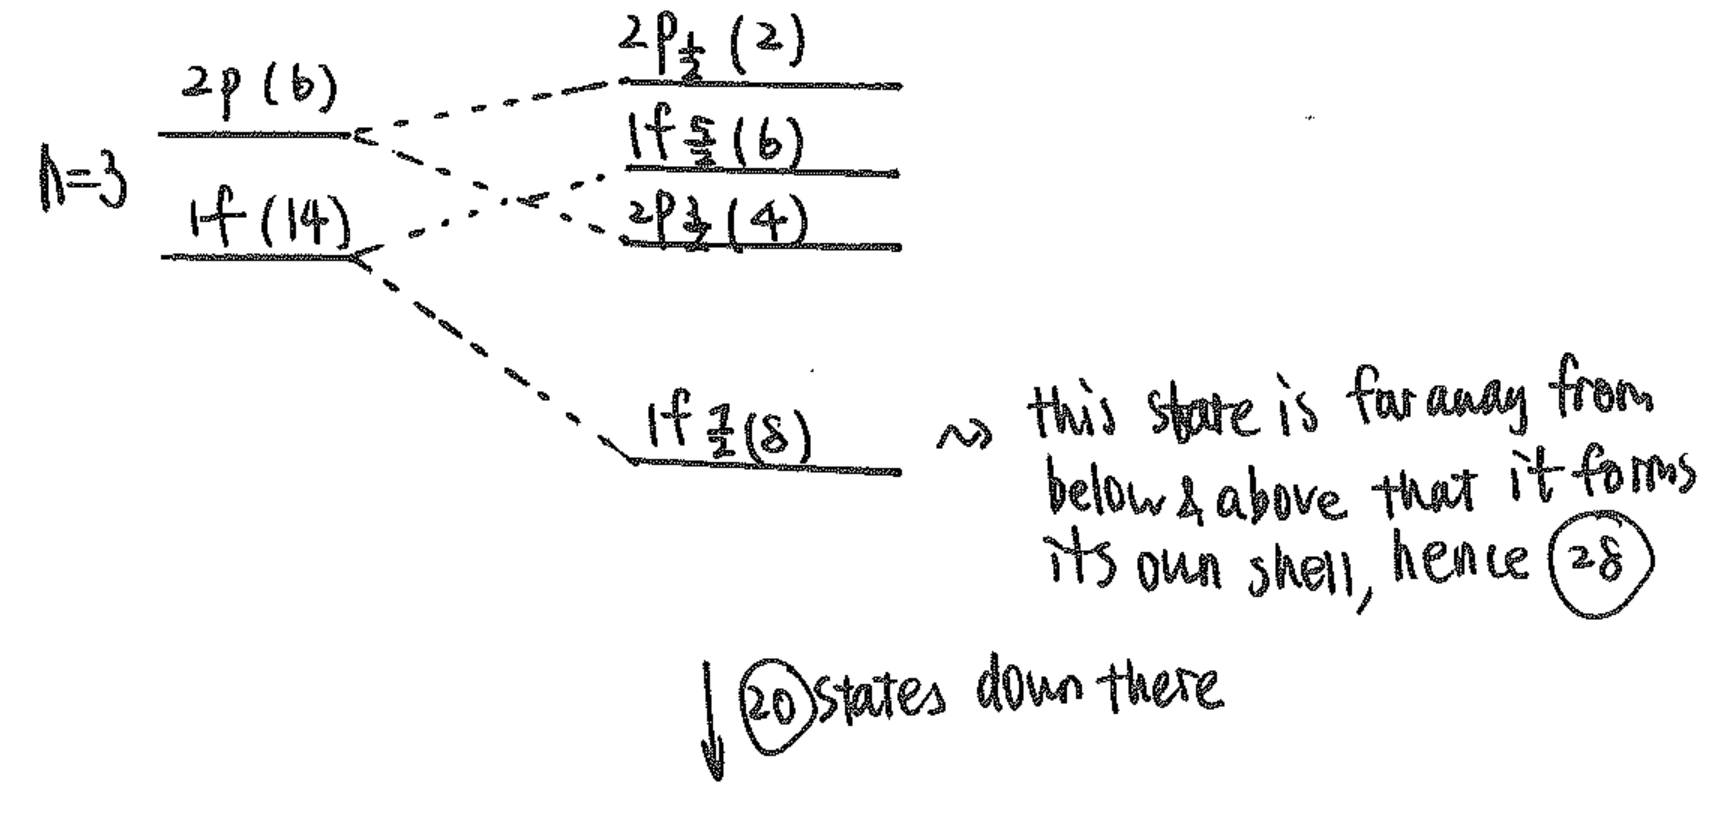
\includegraphics[width=3.5in]{images/shell/magic-number-28.png}
    \caption{Correction to Shell Model $n=3$\label{shell-28}}
\end{figure}

\item $n=4$ oscillator level: Figure~\ref{shell-50}.
\begin{figure}
    \centering
    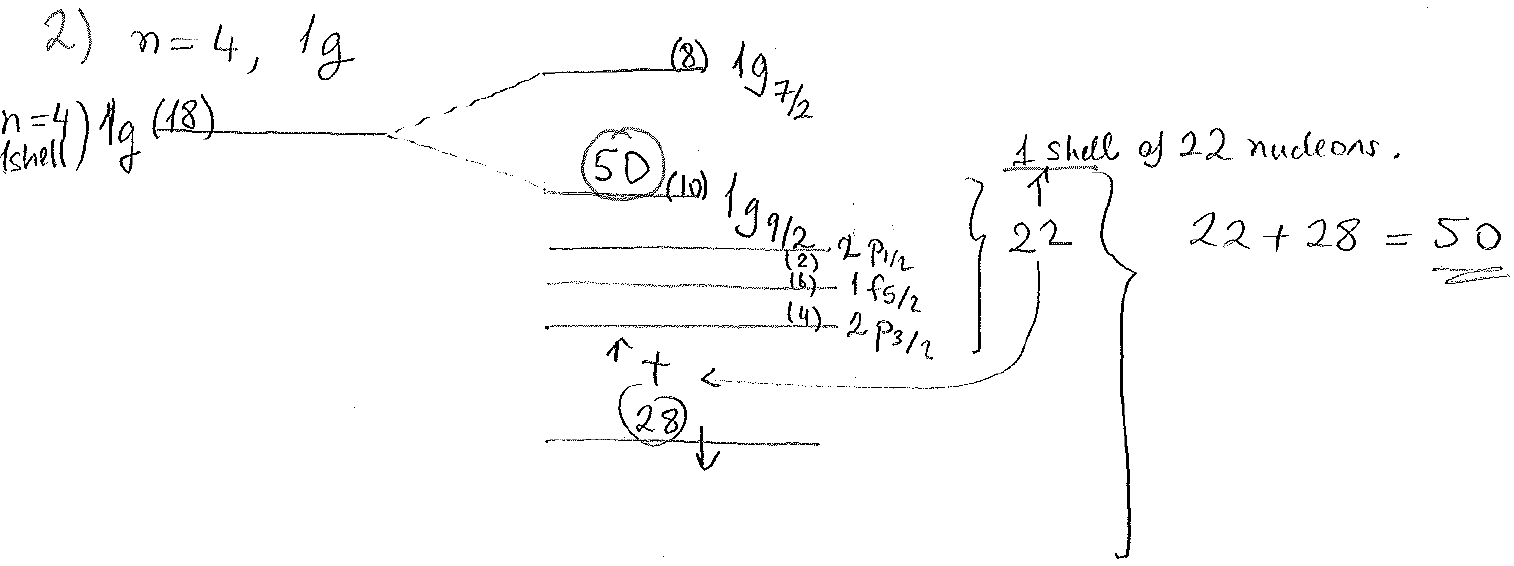
\includegraphics[width=4in]{images/shell/magic-number-50.png}
    \caption{Correction to Shell Model $n=4$\label{shell-50}}
\end{figure}

\item $n=5$ oscillator level: Figure~\ref{shell-82}.
\begin{figure}
    \centering
    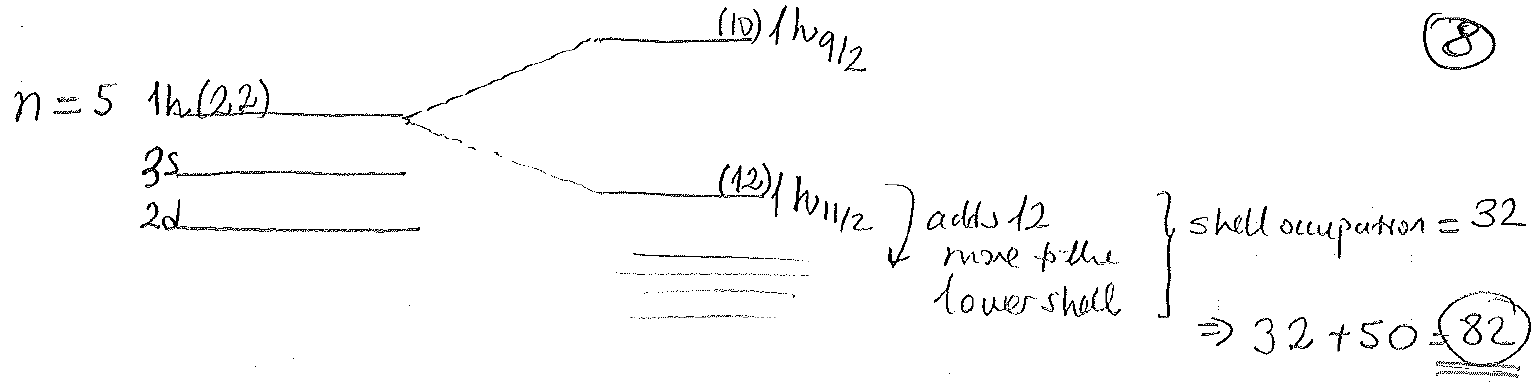
\includegraphics[width=4in]{images/shell/magic-number-82.png}
    \caption{Correction to Shell Model $n=5$\label{shell-82}}
\end{figure}

\item $n=7$ oscillator level: Figure~\ref{shell-126}.
\begin{figure}
    \centering
    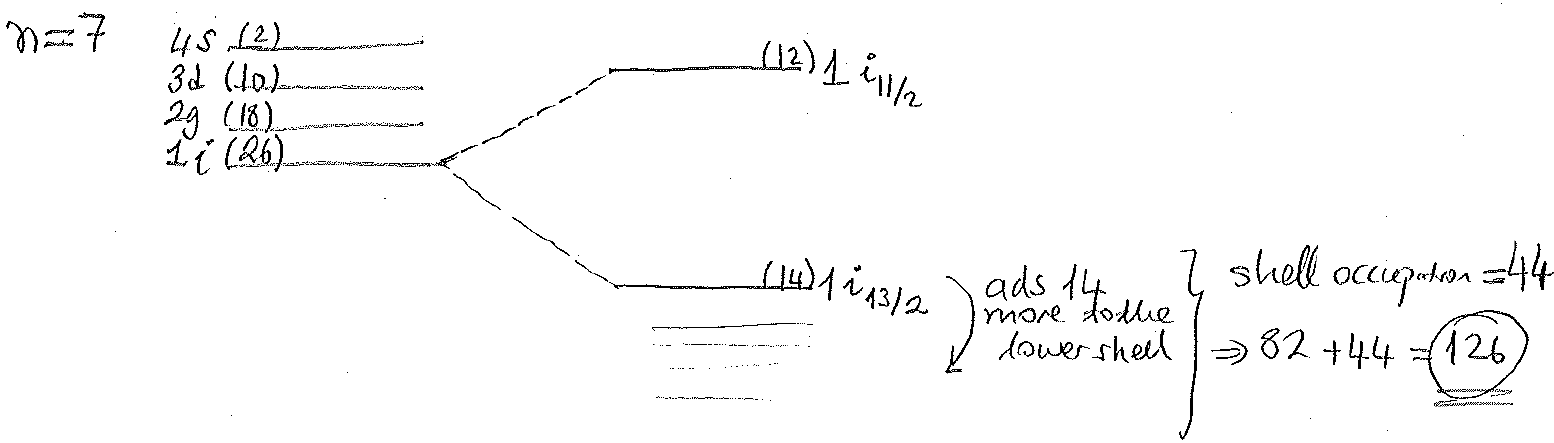
\includegraphics[width=4in]{images/shell/magic-number-126.png}
    \caption{Correction to Shell Model $n=7$\label{shell-126}}
\end{figure}
\end{enumerate}

\uline{Summary}
\begin{enumerate}
\item Know what $l$ values each letter correspond to: $ f \to l=3, g \to l=4$ (starting from $l=0$, the notation goes like: s, p, d, f, h, g). 
\item After knowing $l$, the newly split states are $j= l \pm \frac{1}{2}$, write the new states out as original notation$_{j}$;
\item Degeneracy:$2 j+1$ degeneracy.  
\end{enumerate}


\topic{Ground-state Spin-Parity Assignments/Predictions}
Notation: \ce{^A_p X_n}, proton number determines the type of isotope, neutron number determines isotones.  

We define a \textbf{Total Angular Momentum of Nucleus} to be $I$, and define parity to be $\pi = (-1)^l$. We are going to use the right-hand of Figure~\ref{ns-magic-numbers}.
\begin{figure}[ht]
    \centering
    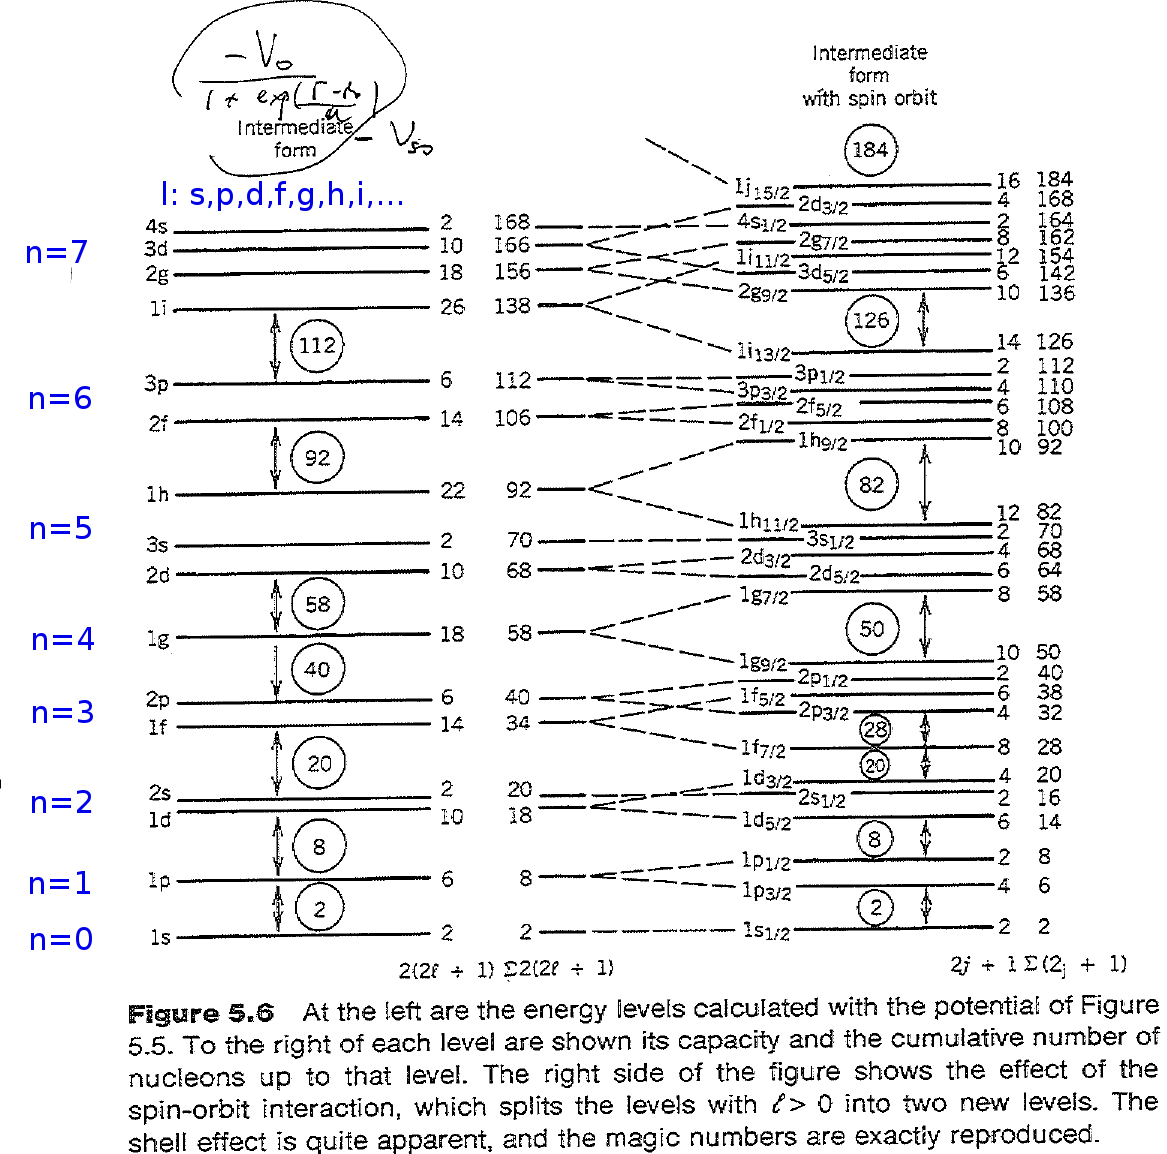
\includegraphics[width=5in]{images/ns/magic-numbers.png}
    \caption{Energy Occupation Diagram}
    \label{ns-magic-numbers}
\end{figure}

\clearpage
\subtopic{Nuclei with Odd A (\# of neutrons plus protons)} 
Example: compare \ce{^{15}_{8}O_7} and \ce{^{17}_8 O_9} in Fig.~\ref{odd-A-nuclide}, we notice that the last nucleon filling the shell model is the one that contributes to the structure. 

\begin{figure}[ht]
  \centering
  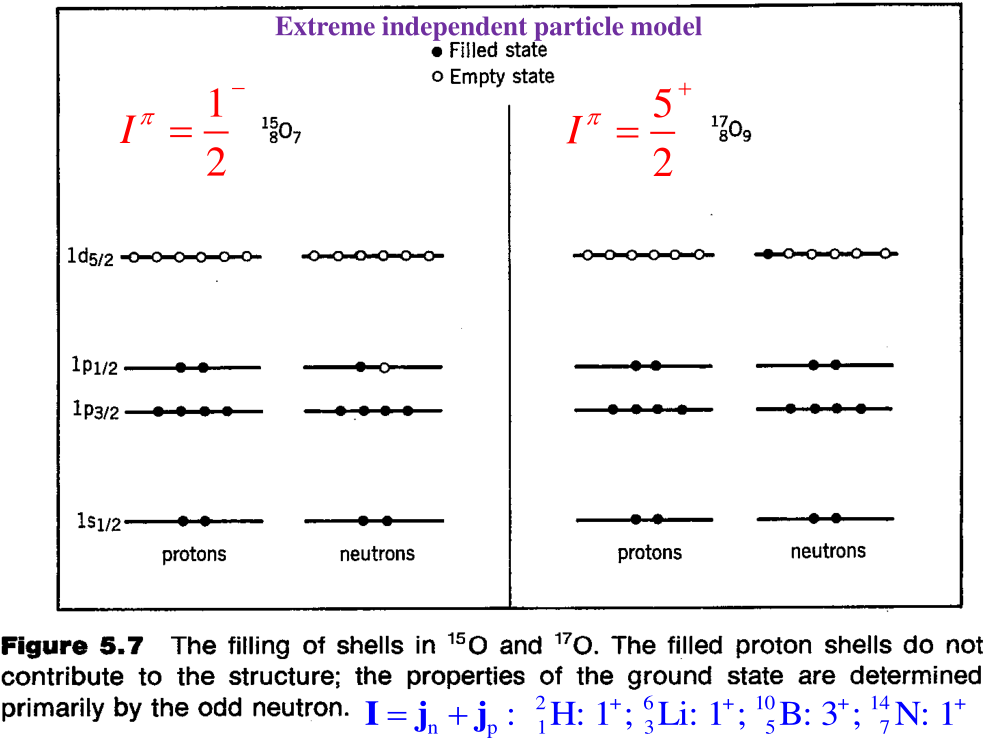
\includegraphics[width=4.5in]{images/ns/odd-A-nuclide.png}
  \caption{The Last Nucleon Contributes To the Structure} \label{odd-A-nuclide}
\end{figure}

Process: 
\begin{enumerate}
\item Determine the number of neutrons, protons from \ce{^A_p X_n};
\item For protons or neutrons whichever is odd, fill in the shell models; do so by start from the bottom level, each level hosts $2j+1$ number of protons; the highest level determines the $l$ value we use to fine $\pi$, and the $j$ value associated with this level is the $I$ term;
\item For now we don't care about the even number nucleons. 
\end{enumerate}

\textbf{Pairing Effect for Larger $l$}: the residual terms we ignored at calculating single-particle Hamiltonian have an effect at short range for nucleons, resulting in a decreased energy and the orbital angular momentum tends to claps to zero. So the state with larger $l$ value is more favored to be filled. 

Example: \ce{^{207}_{82} Pb_{125}}, see Figure~\ref{ns-Pb-125}.
\begin{figure}[ht]
    \centering
    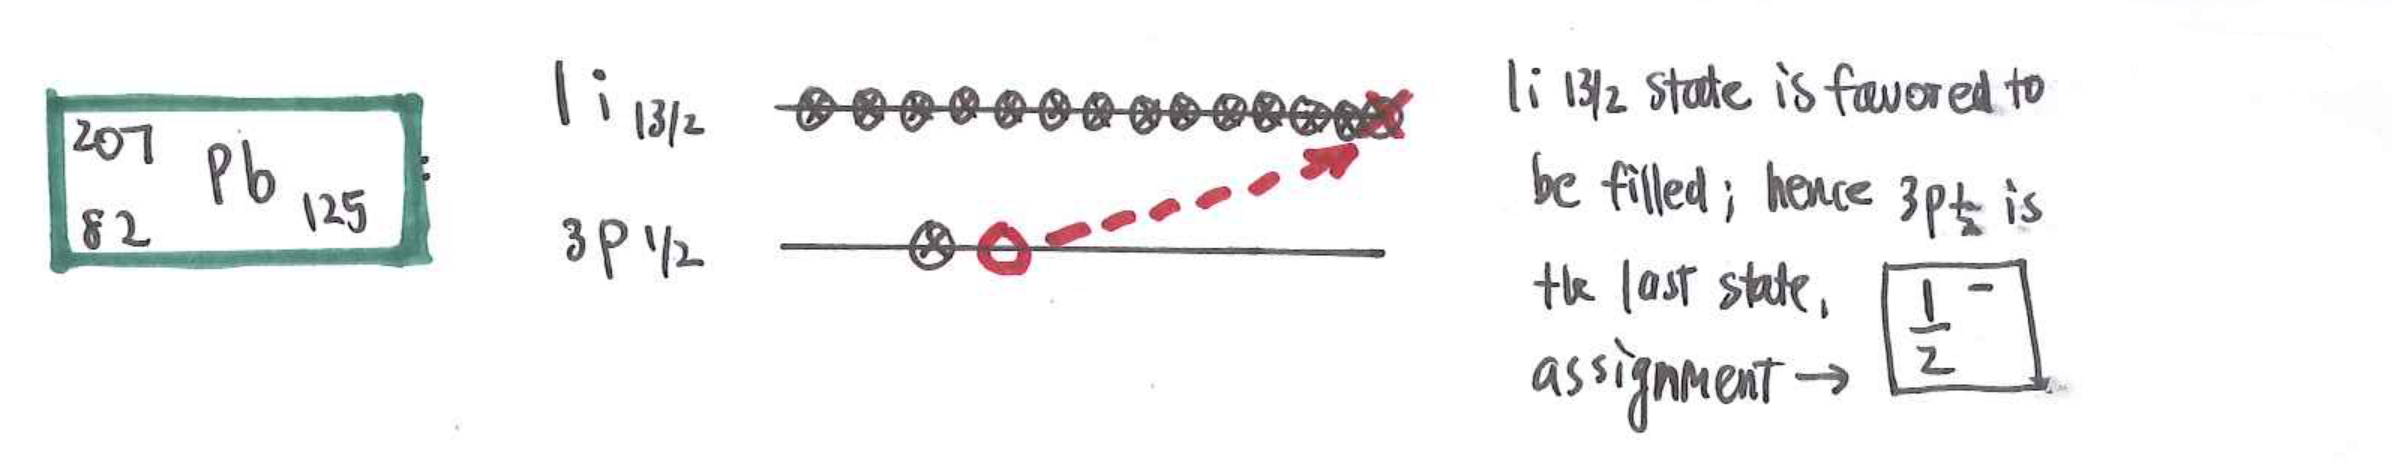
\includegraphics[width=5in]{images/ns/Pb-125.png}
    \caption{Paring Effect Illustration (Odd A): Pb-125}
    \label{ns-Pb-125}
\end{figure}



\subtopic{Even Neutron, Even Proton} 
Derived from the paring effect, nucleons want to minimize the energy by setting the pair's angular momentum to zero. Among the hundreds of stable or radioactive even-Z even-N nuclides, all have $I=0$. This is strong evidence for the nuclear paring force. Example: \ce{^{40}_{20}Ca_{20}}, \ce{^{36}_{18} A_{18}}, \ce{^{130}_{36} Sn_{80}}, $\cdots$. 


\subtopic{Odd Neutron, Odd Proton}
There are only 4 stable odd-Z odd-N nuclides: \ce{_1 H_1}, \ce{_3 Li_3}, \ce{_5 B_5}, \ce{_7 N_7}. 


There is a tendency to align the spin of the last neutron state and the last proton state. We can flip either state, as long as we take the magnitude of the resulting $I$. See approach one of \ce{^{38} Cl_{21}} in Figure~\ref{ns-Cl-21}.
\begin{figure}[ht]
    \centering
    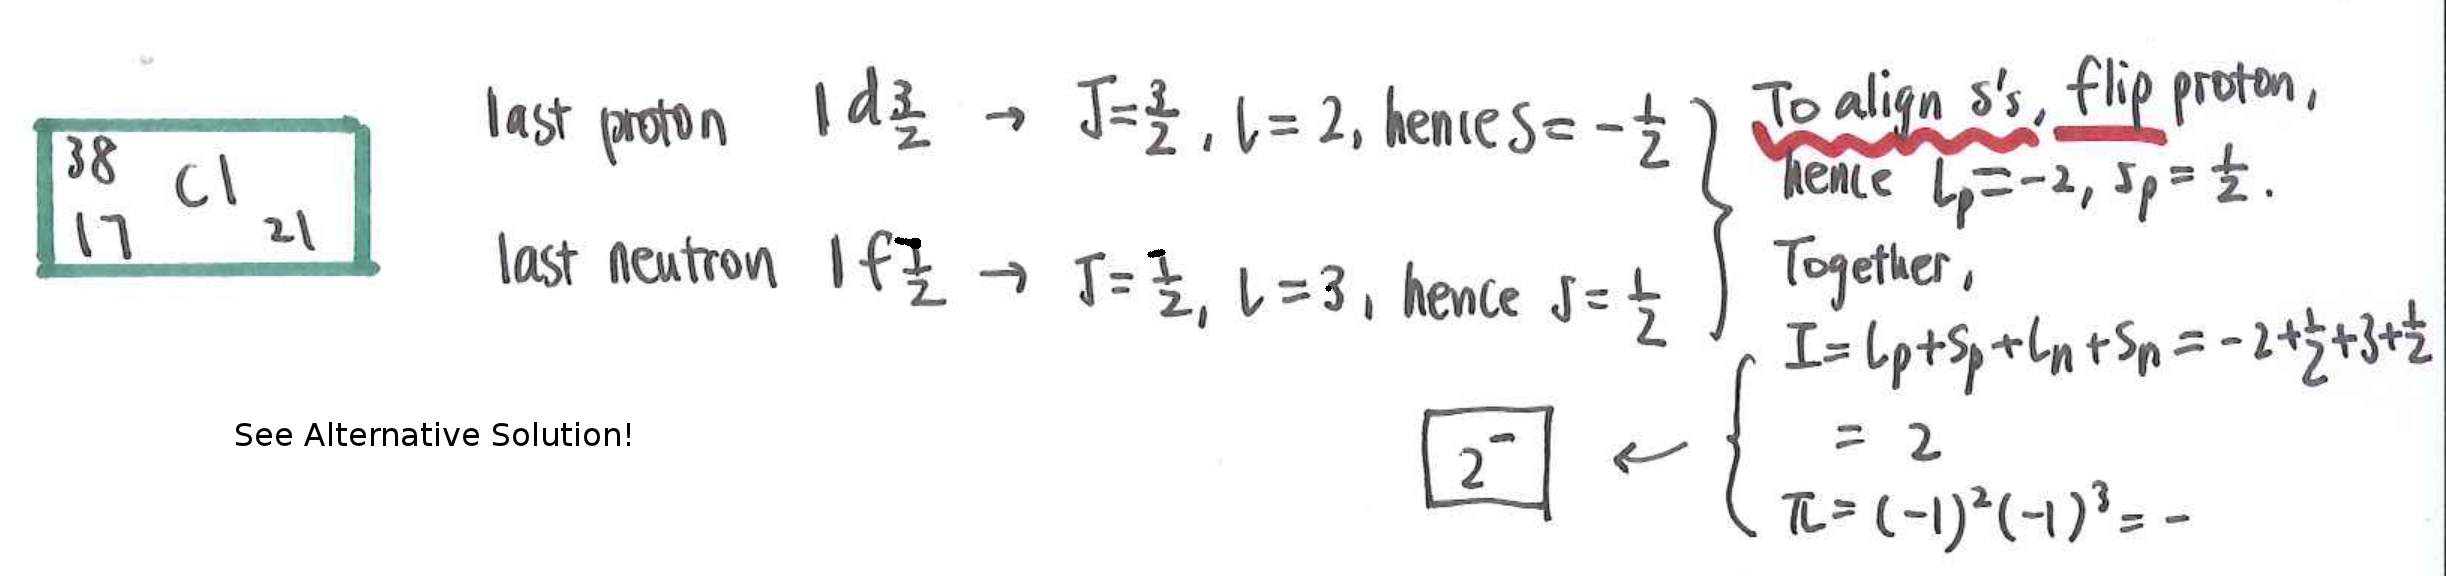
\includegraphics[width=5in]{images/ns/Cl-21.png}
    \caption{Flip Spin Effect Illustration (Odd-Odd): Cl-21}
    \label{ns-Cl-21}
\end{figure}

Alternative approach: Again we look at the last neutron and last proton, which are $1d_{3/2}, 1f_{7/2}$. Immediately we know $ \frac{7}{2} - \frac{3}{2} \le I \le \frac{7}{2} + \frac{3}{2}$. Consider Table~\ref{spin-l}, we know one is spin up, one is spin down, that is suggesting, we pick the opposite case for $I$, that is, $I=\frac{7}{2} - \frac{3}{2} =2$. The spin part is $(-1)^{L_p} (-1)^{L_n} = (-1)^3 (-1)^2 = -1$. Hence the result is $2^-$.  
\begin{table}[ht]
\centering
\begin{tabular}{|c|c|c|} \hline
l & spectro & Spin \\ \hline
0 & s & + \\ \hline
1 & p & - \\ \hline
2 & d & + \\ \hline
3 & f & - \\ \hline
4 & g & + \\ \hline
\end{tabular}
\caption{Spin Based on $l$\label{spin-l}}
\end{table}



\end{document}
